\documentclass[12pt]{article}

\usepackage{sbc-template}
\usepackage{graphicx,url}
\usepackage[utf8]{inputenc}
\usepackage[brazil]{babel}
%\usepackage[latin1]{inputenc}

     
\sloppy

\title{Avaliação de desempenho da implementação paralela do método CSEM 3D no supecomputador Santos Dumont}

\author{Mateus F. L. de Souza\inst{1,2}, Rômulo T. Lima\inst{1,3}}

\address{  Laboratório Nacional de Computação Científica (LNCC)\\
  Getúlio Vargas Av., 333, Quitandinha Petrópolis - RJ - Brasil
\nextinstitute
  Centro Federal de Educação Tecnológica Celso Suckow da Fonseca (CEFET-FR) \\
  R. Gen. Canabarro, 485 - Maracanã, Rio de Janeiro - RJ - Brasil
\nextinstitute
Universidade Católica de Petrópolis (UCP)\\
  R. Barão do Amazonas, 124 - Centro, Petrópolis - RJ - Brasil  
  \email{\{facanha,romulotl\}@lncc.br}
}

\begin{document} 

\maketitle

\begin{abstract}
  This work presents the results of parallel execution on the Santos Dumont supercomputer implementing CSEM 3D method. To this end, concepts and methods of implementing parallel processing were developed, operating with a high level of computational resources. Through this,  empirically, it was possible  to verify that the operation of a large amount of resources is not synonymous with efficiency.
\end{abstract}
     
\begin{resumo} 
  Este trabalho apresenta os resultados obtidos pela execução paralela no supercomputador Santos Dumont na implementação do método CSEM 3D. Para tal foram desenvolvidos conceitos e métodos de implementação de processamento paralelo, operando com grande nível de recursos computacionais. Com isso foi possível constatar empíricamente que a operação de grande quantidade de recursos não é sinônimo de eficiência.
\end{resumo}

\section{Introdução}
Este trabalho tem como objetivo explorar a eficiência da paralelização no código CSEM 3D, utilizando como ferramenta o OpenMPI, observando tabém a forma como os recursos computacionais foram utilizados de 1 até 384 nós computacionais. O experimento consiste na confecção de duas linhas, apresentando a média de tempo de execução do código CSEM 3D, uma das linhas apresentando no máximo 24 processos MPI por nó computacional. Já na outra linha, apresentando um máximo de 48 processos por nó computacional.

\section{CSEM} \label{sec:firstpage}
Controlled-Source Eletromagnetic (CSEM) é um método de mapeamento geofisico, empregando um monitoramento eletromagnético através de sensores remotos que mapeia a resistência elétrica da superfície aquática. Este método é utilizado em larga escala por diversas aplicações na área mineral (Castillo-Reyes
Octavio et al, Sheard et al.2005 2019). Estudos de condutividade de cristais (Castillo-Reyes
Octavio et al; Hördt et al.1992, 2019). Além disso, realiza uma caracterização do armazenamento de CO2 (Castillo-Reyes
Octavio et al; Girard et al.2019). Indo além, faz a projeção de reservatório geotérmico (Castillo-Reyes
Octavio et al; Coppo et al.2019) e exploração de hidrocarboneto, utilizando tecnologia embarcada (Castillo-Reyes
Octavio et al; Newman \& Alumbaugh 1997; Eidesmo et al.2002; Avdeev 2005; Constable 2006; Srnka et al.2006; Orange et al.2009; Börner 2010; Constable 2019). 
\section{Processamento Paralelo}
(Philippe O. A. Navaux)É uma forma eficiente de processamento da informação com ênfase na exploração de eventos concorrentes no processo computacional. 
O processamento paralelo existe a partir do momento em que dois ou mais processadores interagem entre si para resolverem uma determinada tarefa. Por tanto este assunto é muito vasto e implica desde algoritmos que possam ser paralelizados, até as arquiteturas paralelas. É importante salientar que paralelismo não implica necessariamente em máquinas de alta performance, conhecidos como supercomputadores, mas trata também do paralelismo em situações de baixa velocidade; claro que usualmente quando se fala de paralelismo estamos tratando do primeiro caso, como o desde trabalho que estamos utilizando o supercomputador Santos Dumont.


\section{Resultados}
Nesta sessão apresentaremos os resultados da implementação dos trabalhando encima dos conceitos trabalhados neste artigo.
Foram feitas duas linhas apresentando a média de 4 rodadas por ponto na linha para para gerar um resultado próximo da realidade.
Para a paralelização foi utilizado o OpenMPI fazendo linhas que divergem em relação ao máximo de processos por nó computacional, uma limitada em 48 processos (figura 2). Enquanto a outra, limitada em 24 processos (figura 3).

\begin{figure}[ht]
\centering
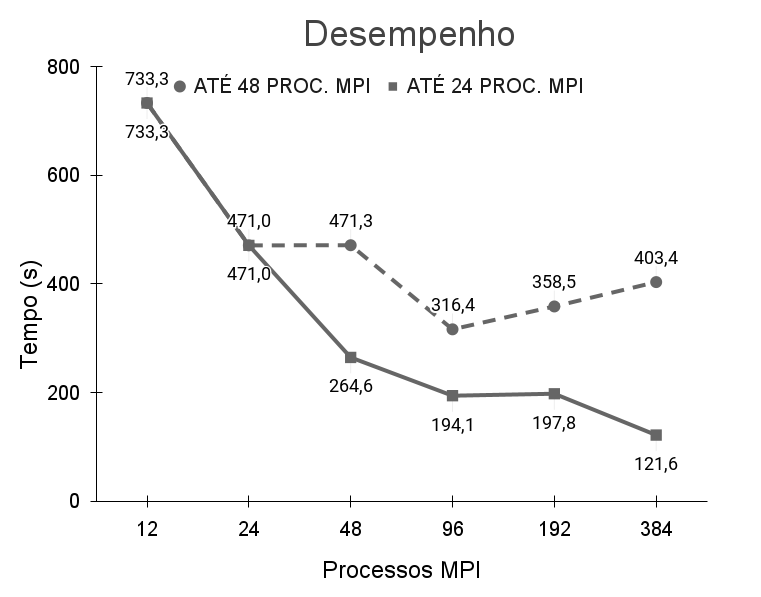
\includegraphics[width=.5\textwidth]{figures/perfpernode.png}
\caption{Está imagem apresenta um comparativo entre as linhas de média de 24 e 48 processos MPI por nó.}
\label{fig:48pernode}
\end{figure}

\begin{figure}[ht]
\centering
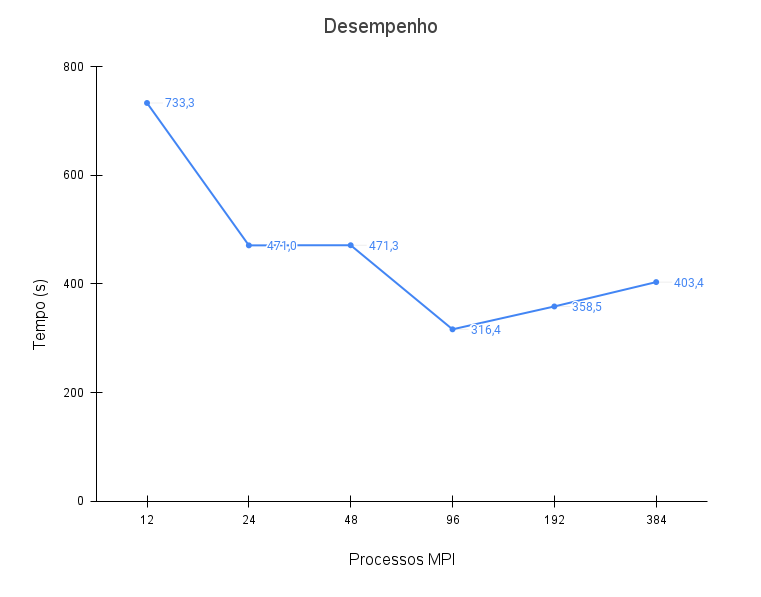
\includegraphics[width=.5\textwidth]{figures/perfupto48pernode.png}
\caption{Nessa imagem foi foram executados jobs utilizando respectivamente: 1, 1, 1, 2, 4, 8 nós computacionais e no máximo 48 processos por nó.}
\label{fig:48MPI}
\end{figure}

\begin{figure}[ht]
\centering
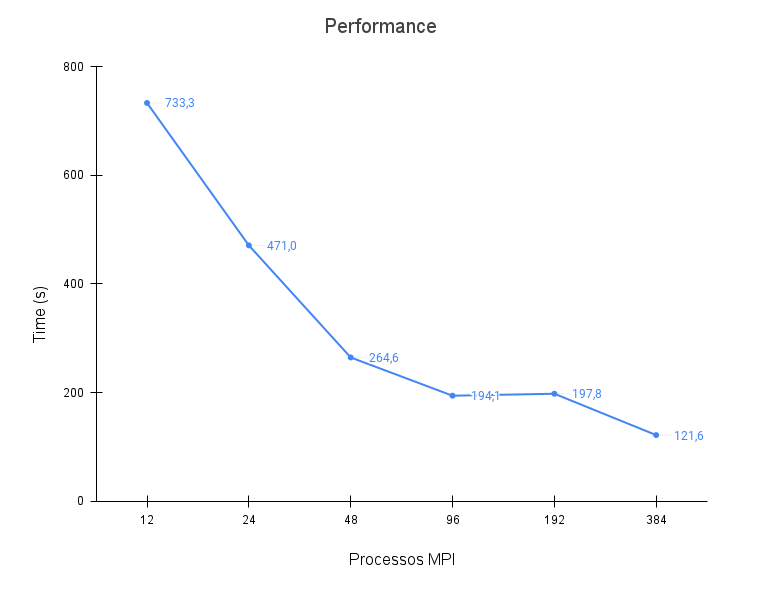
\includegraphics[width=.5\textwidth]{figures/perfupto24pernode.png}
\caption{Nessa imagem foi foram executados jobs utilizando respectivamente: 1, 1, 2, 4, 8, 16 nós computacionais e no máximo 24 processos por nó.}
\label{fig:24MPI}
\end{figure}

\section{Comentários}


Bibliographic references must be unambiguous and uniform.  We recommend giving
the author names references in brackets, e.g. \cite{knuth:84},
\cite{boulic:91}, and \cite{smith:99}.

$$

  Castillo-Reyes, Octavio, et al. “Parallel 3-D Marine Controlled-Source Electromagnetic Modelling Using High-Order Tetrahedral Nédélec Elements.” Geophysical Journal International, vol. 219, no. 1, Oct. 2019, pp. 39–65, https://doi.org/10.1093/gji/ggz285.

  Introdução ao Processamento Paralelo
  Philippe O. A. Navaux
  https://doi.org/10.5753/sbac-pad.1988.23511

$$
The references must be listed using 12 point font size, with 6 points of space
before each reference. The first line of each reference should not be
indented, while the subsequent should be indented by 0.5 cm.

\bibliographystyle{sbc}
\bibliography{sbc-template}

\end{document}
